\documentclass[11pt,a4paper]{article}
\newcommand{\gls}[1]{#1\textsubscript{G}}
\usepackage[utf8]{inputenc}
\usepackage[italian]{babel}
\usepackage{geometry}
\usepackage{graphicx}
\usepackage{float}
\usepackage{tabularx}
\usepackage{booktabs}
\usepackage{hyperref}
\usepackage{fancyhdr}
\usepackage{lastpage}
\usepackage{tikz}
\usepackage{pgf-pie}

\geometry{margin=2.5cm}

% Intestazione e piè di pagina
\pagestyle{fancy}
\fancyhf{}
\renewcommand{\headrulewidth}{0pt}
\fancyfoot[C]{\thepage\ di \pageref{LastPage}}

\begin{document}

% Prima pagina - Intestazione
\begin{titlepage}
    \centering
    
    % Logo Università
    \begin{figure}[H]
        \centering
        
\includegraphics[width=0.3\textwidth]{../logoUnipd.jpg}
    \end{figure}
    
    \vspace{0.5cm}
    
    \textbf{\Large Università degli Studi di Padova} \\
    \vspace{0.2cm}
    \textbf{Laurea in Informatica} \\
    \vspace{0.2cm}
    \textbf{Corso di Ingegneria del Software} \\
    \vspace{0.2cm}
    \textbf{Anno Accademico 2025/2026} \\
    
    \vspace{1cm}
    
    % Logo gruppo
    \begin{figure}[H]
        \centering
        
\includegraphics[width=0.2\textwidth]{../LogoByteMe.jpg}
    \end{figure}
    
    \vspace{0.5cm}
    
    \textbf{\Large Gruppo ByteMe} \\
    \vspace{0.2cm}
    \texttt{byteme2025swe@gmail.com} \\
    
    \vspace{1cm}
    
    \textbf{\Huge \gls{Manuale Utente}} \\
    
\vspace{1.5cm}
    
    \begin{table}[H]
        \centering
        \begin{tabular}{|l|p{5cm}|}
            \hline
            \textbf{Versione} & 0.1.0 \\
            \hline
            \textbf{Stato} & In corso\\
            \hline
            \textbf{Redazione} & Giulia Barzon\\
            \hline
            \textbf{\gls{Verifica}} & Verificato \\
            \hline
            \textbf{Approvazione} & \\
            \hline
            \textbf{Proprietario} & ByteMe \\
            \hline
            \textbf{Uso} & Esterno \\
            \hline
            \textbf{Destinatari} & Prof. Tullio Vardanega \\ & Prof. Riccardo Cardin \\
            \hline
        \end{tabular}
    \end{table}
    
    \vfill
\end{titlepage}

% Seconda pagina - Versionamento
\thispagestyle{empty}
\section*{Registro dei Cambiamenti}

\begin{table}[H]
    \centering
    \begin{tabular}{|c|c|c|>{\raggedright\arraybackslash}p{0.35\textwidth}|p{0.18\textwidth}|}
        \hline
        \textbf{Versione} & \textbf{Data} & \textbf{Autore} & \textbf{Descrizione} & \textbf{\gls{Verifica}} \\
        \hline
        0.1.0 & 24/04/2026 & Giulia Barzon & Completate sezioni 1,2,3 e bozza di tutte le altre sezioni & \\
        \hline
        0.0.1 & 01/04/2026 & Giulia Barzon & Creazione del documento, scrittura introduzione & Tommaso Tombacco \\
        \hline
    \end{tabular}
    \caption{Registro delle versioni del documento}
    \label{tab:versionamento}
\end{table}

\newpage

% Terza pagina - Indice
\tableofcontents
\thispagestyle{empty}
\newpage

% Dalla quarta pagina - Contenuto principale
\setcounter{page}{1}

\section{Introduzione}
\subsection{Scopo del documento}
Lo scopo del presente documento è fornire all'utente finale tutte le istruzioni necessarie per l'installazione, la configurazione e l'utilizzo corretto del software \textbf{"Second Brain"}.  Il manuale include i requisiti di sistema, una guida all'avvio tramite \gls{Docker} e una descrizione dettagliata di tutte le funzionalità offerte dall'interfaccia web, supportata da screenshot esplicativi.

\subsection{Scopo del prodotto}
Il progetto "Second Brain" si propone di rivoluzionare il processo di scrittura e organizzazione delle idee integrando modelli linguistici di grandi dimensioni (LLM) in un \gls{editor di testo} \gls{Markdown} moderno. 
Il sistema offre funzionalità avanzate tra cui:
\begin{itemize}
    \item \textbf{Editor \gls{Markdown}:} Scrittura con anteprima in tempo reale.
    \item \textbf{Analisi critica:} Sistema di revisione del testo basato sulla metodologia dei "Sei Cappelli per Pensare" di Edward De Bono.
    \item \textbf{\gls{Distant writing}:} Generazione di testi completi a partire da brevi \gls{prompt}.
    \item \textbf{Elaborazione AI:} Funzioni di riassunto, riscrittura, traduzione e correzione grammaticale automatica.
\end{itemize}

L’obiettivo è creare uno strumento di supporto alla scrittura creativa, esplorando le potenzialità degli LLM nel contesto del note-taking avanzato.

\subsection{Target di utenti}
Il prodotto è progettato per essere accessibile anche senza competenze tecniche avanzate ed è rivolto a:
\begin{itemize}
    \item \textbf{Studenti}: per la stesura di appunti, riassunti e materiale di studio
    \item \textbf{Professionisti}: per la creazione di documenti aziendali, report e presentazioni
    \item \textbf{Scrittori e content creator}: per l'ideazione, stesura e revisione di contenuti
    \item \textbf{Ricercatori}: per l'organizzazione di appunti di ricerca e letteratura
    \item \textbf{Utenti generici}: chiunque abbia bisogno di un editor per esigenze di scrittura assistita
\end{itemize}


\subsection{\gls{Glossario}}
Per evitare ambiguità, i termini tecnici usati nel documento vengono definiti in modo più approfondito nel documento \gls{Glossario} v2.0.0 che si può trovare nel sito web del gruppo ByteMe alla sezione Documenti Interni e raggiungibile dal seguente link:\\
\href{https://byteme25.github.io/ByteMe/files.html}{ByteMe/\gls{Glossario} v2.0.0}

I termini che vengono considerati meritevoli di approfondimenti sono indicati con una G a pedice.


\subsection{Riferimenti}
\subsubsection{Riferimenti normativi}
\begin{itemize}
  \item \textit{\gls{Norme di Progetto}} versione 2.0.0\\
  \href{https://byteme25.github.io/ByteMe/files.html}{ByteMe/\gls{Norme di Progetto} v2.0.0}
  \item Capitolato d'appalto C6: \textit{Second Brain} (Zucchetti S.p.A.)\\ \url{https://www.math.unipd.it/~tullio/IS-1/2025/Progetto/C6.pdf}
  \item Regolamento del progetto didattico:\\
        \url{https://www.math.unipd.it/~tullio/IS-1/2023/Dispense/PD2.pdf}
\end{itemize}

\subsubsection{Riferimenti informativi}
\begin{itemize}
    \item \gls{Glossario} v2.0.0 (Ultimo accesso: 01/04/2026)\\
    \href{https://byteme25.github.io/ByteMe/files.html}{ByteMe/\gls{Glossario} v2.0.0}
\end{itemize}

\newpage

\section{Requisiti di sistema}
Per garantire un'esperienza d'uso ottimale e il corretto funzionamento di tutte le funzionalità basate sull'intelligenza artificiale, è necessario che l'ambiente di esecuzione rispetti i requisiti minimi descritti di seguito.

\subsection{Browser supportati}
L'applicazione è una Web App accessibile tramite browser. Per una corretta visualizzazione dell'interfaccia e la gestione delle chiamate asincrone, si consiglia l'utilizzo delle versioni più recenti dei seguenti browser:
\begin{itemize}
    \item \textbf{Google Chrome:} Versione 110 o superiore;
    \item \textbf{Mozilla Firefox:} Versione 115 o superiore;
    \item \textbf{Microsoft Edge:} Versione 110 o superiore;
    \item \textbf{Safari:} Versione 16 o superiore.
\end{itemize}

\subsection{Requisiti Hardware}
Sebbene l'elaborazione dei modelli linguistici ($LLM_G$) avvenga su server remoti, la gestione locale dei container \gls{Docker} e dell'interfaccia richiede le seguenti specifiche minime, considerate sufficienti per l'utilizzo scorrevole dell'applicazione:
\begin{itemize}
    \item \textbf{Processore (CPU):} Architettura x86-64 o ARM64, minimo 2 core;
    \item \textbf{Memoria RAM:} Almeno 8 GB (consigliati 16 GB per l'esecuzione fluida di \gls{Docker} Desktop e del browser contemporaneamente);
    \item \textbf{Spazio su disco:} Circa 2 GB di spazio libero per le immagini \gls{Docker} e i volumi del \gls{database} \gls{PostgreSQL}.
\end{itemize}

\subsection{Requisiti software}
Trattandosi di un'applicazione distribuita tramite container, l'unico software richiesto per l'installazione è \textbf{\gls{Docker}} (comprensivo di \gls{Docker} Compose).
\begin{itemize}
    \item \textbf{Per utenti Windows/Mac}: Si consiglia l'installazione di \textit{Docker Desktop}.
    \item \textbf{Per utenti Linux}: Assicurarsi che il servizio \texttt{docker} sia attivo e che l'utente disponga dei permessi necessari per eseguire \texttt{docker-compose}.
\end{itemize}

\subsection{Connessione Internet}
È necessaria una \textbf{connessione Internet stabile} per permettere al sistema di comunicare con i servizi di intelligenza artificiale. Una connessione lenta potrebbe aumentare i tempi di attesa per la generazione dei testi e per le funzionalità di AI sul testo.


\newpage

%  =================================================================
% Installare Docker e preparare l'ambiente per eseguire Second Brain
%  =================================================================
\section{Installazione e avvio}
In questa parte del manuale viene illustrato come installare e avviare \textbf{"Second Brain"} sul proprio computer. Sebbene la destinazione finale del prodotto sia l'esecuzione su server dedicati dell'azienda proponente, la configurazione in locale è il modo più rapido per esplorarne le funzionalità.

Per utilizzare \textbf{Second Brain} sul proprio computer, il metodo più semplice è l'utilizzo di \textbf{\gls{Docker}}. Questa tecnologia permette di "impacchettare" tutto il software necessario in contenitori pronti all'uso, evitando di dover installare manualmente \gls{database} o linguaggi di programmazione specifici.

\subsection{Installazione di \gls{Docker} Desktop}
Prima di tutto, è necessario installare il programma principale sul proprio computer:
\begin{enumerate}
    \item Visita il sito ufficiale: \href{https://www.docker.com/products/docker-desktop/}{\gls{docker}.com/products/\gls{docker}-desktop};
    \item Scarica la versione adatta al tuo sistema operativo (Windows, Mac o Linux);
    \item Avvia l'installatore e segui le istruzioni a schermo;
    \item Al termine dell'installazione, riavvia il computer se richiesto e apri l'applicazione \textbf{\gls{Docker} Desktop}.
\end{enumerate}

\subsection{Preparazione dei file}
Una volta installato \gls{Docker}, apri il terminale (o il \gls{prompt} dei comandi) e posizionati nella cartella dove desideri salvare il progetto. Digita il seguente comando per scaricare i file:
\begin{center}
    \texttt{\gls{git} clone https://\gls{github}.com/ByteMe25/PB\_ByteMe}
\end{center}
Successivamente, entra nella cartella del progetto:
\begin{center}
    \texttt{cd PB\_ByteMe}
\end{center}

\subsection{Configurazione delle chiavi API}
Affinché le funzioni di Intelligenza Artificiale siano operative, è necessario fornire al sistema le credenziali di accesso ai modelli linguistici.
\begin{enumerate}
    \item Individua nella cartella principale il file denominato \texttt{.env.example}.
    \item Crea una copia del file e rinominala esattamente in \texttt{.env}.
    \item Apri il file \texttt{.env} con un editor di testo e compila i campi richiesti:
    \begin{itemize}
        \item \texttt{OPENAI\_API\_KEY}: Inserisci la tua chiave segreta fornita dal provider (es. Zucchetti o OpenAI).
        \item \texttt{OPENAI\_BASE\_URL}: Inserisci l'indirizzo del server che eroga i modelli.
        \item \texttt{FLASK\_SECRET\_KEY}: Inserisci una stringa casuale a tua scelta per mettere in sicurezza le sessioni tecniche del server.
    \end{itemize}
\end{enumerate}

\subsection{Comandi di avvio}
Con il terminale aperto nella cartella del progetto, digita il seguente comando:
\begin{center}
    \texttt{\gls{docker}-compose up --build}
\end{center}
Il sistema inizierà a scaricare i componenti necessari. Questo processo può richiedere diversi minuti durante il primo avvio. Quando il testo nel terminale indicherà che i servizi \textit{backend} e \textit{frontend} sono attivi, l'applicazione è pronta.


\subsection{Accesso al software}
A installazione completata, non chiudere la finestra del terminale. Apri il tuo browser preferito e digita nella barra degli indirizzi:
\begin{center}
    \textbf{http://localhost:8080}
\end{center}
Verrai reindirizzato immediatamente all'interfaccia di Second Brain e potrai iniziare a scrivere i tuoi documenti.

\subsection{Spegnimento}
Per chiudere l'applicazione e liberare risorse sul computer, torna nella finestra del terminale e premi contemporaneamente i tasti \textbf{Ctrl + C}. Una volta che il testo smette di scorrere, puoi chiudere la finestra.


\newpage

% ==========================================
% GUIDA ALL'INTERFACCIA
%===========================================
\section{Guida all'interfaccia}
L'interfaccia di \textit{Second Brain} è progettata per ridurre al minimo le distrazioni, mettendo al centro il contenuto testuale. Lo spazio di lavoro è suddiviso in tre aree principali: la barra superiore (\textit{Topbar}), la barra laterale (\textit{Sidebar}) e l'area di scrittura centrale.

\begin{figure}[H]
    \centering
    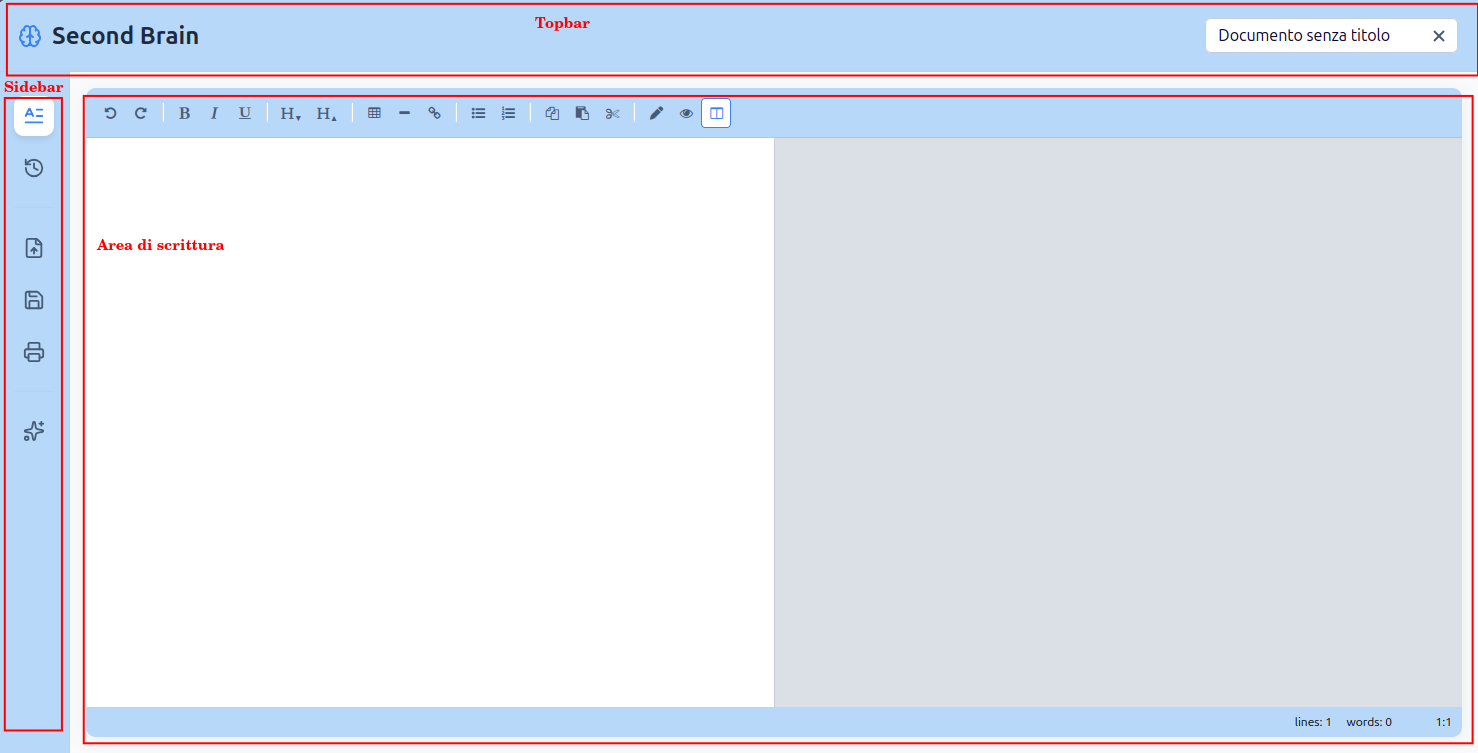
\includegraphics[width=1\textwidth]{../ManualeUtenteimg/schermata_iniziale.png}
    \caption{Panoramica dell'interfaccia di Second Brain: Topbar, Sidebar, area di testo dell'Editor.}
    \label{fig:panoramica}
\end{figure}

\subsection{La barra superiore (Topbar)}
La \textit{Topbar} permette di gestire l'identità del documento corrente.
\begin{itemize}
    \item \textbf{Titolo del documento}: Cliccando sul nome del documento presente in alto a destra, è possibile rinominare il file in tempo reale. Il nome scelto verrà utilizzato come nome predefinito durante l'esportazione.
    \item \textbf{Chiusura del documento}: Cliccando sulla X accanto al nome del documento è possibile chiudere il file corrente.
\end{itemize}

\textit{Nota}: Il sistema monitora costantemente le modifiche: un avviso di sicurezza impedirà la chiusura accidentale del browser o del documento se sono presenti dati non ancora salvati.

\begin{figure}[H]
    \centering
    % Prima immagine (a sinistra)
    \begin{minipage}[b]{0.48\textwidth}
        \centering
        
\includegraphics[width=\textwidth]{../ManualeUtenteimg/titolo_doc.png}
        \caption{Topbar: Titolo del documento}
        \label{fig:titolo_documento}
    \end{minipage}
    \hfill % Inserisce uno spazio elastico tra le due immagini
    % Seconda immagine (a destra)
    \begin{minipage}[b]{0.48\textwidth}
        \centering
        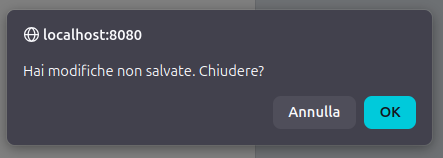
\includegraphics[width=\textwidth]{../ManualeUtenteimg/avviso_chiusura.png}
        \caption{Avviso di chiusura documento}
        \label{fig:avviso_chiusura_doc}
    \end{minipage}
\end{figure}

\subsection{La barra laterale (Sidebar)}
Posizionata a sinistra, la \textit{Sidebar} è il centro operativo del software. Contiene i comandi per la navigazione e le funzioni principali:
\begin{itemize}
    \item \textbf{Navigazione}: Permette di passare rapidamente dalla vista "Editor" alla vista "Storico delle generazioni".
    \item \textbf{Azioni AI}: Apre il pannello dedicato agli strumenti di Intelligenza Artificiale.
    \item \textbf{Gestione file}: Icone dedicate per il caricamento (\textit{Upload}) di file locali e per il salvataggio/esportazione del lavoro.
    \item \textbf{Stampa}: Avvia la funzione di stampa del browser ottimizzata per il documento corrente.
\end{itemize}

\begin{figure}[H]
    \centering
    % Prima immagine (Sinistra) - Navigazione
    \begin{minipage}[b]{0.30\textwidth}
        \centering
        
\includegraphics[width=\textwidth]{../ManualeUtenteimg/sidebar_navigazione.png}
        \caption{Navigazione}
        \label{fig:sidebar_navigazione}
    \end{minipage}
    \hfill
    % Seconda immagine (Centro) - Gestione File
    \begin{minipage}[b]{0.30\textwidth}
        \centering
        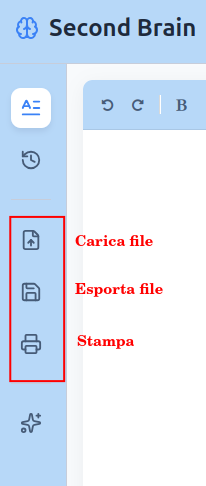
\includegraphics[width=\textwidth]{../ManualeUtenteimg/sidebar.png}
        \caption{Gestione file}
        \label{fig:sidebar_gestione_file}
    \end{minipage}
    \hfill
    % Terza immagine (Destra) - Funzionalità AI
    \begin{minipage}[b]{0.30\textwidth}
        \centering
        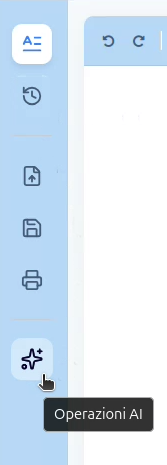
\includegraphics[width=\textwidth]{../ManualeUtenteimg/sidebar_ai.png}
        \caption{Azioni AI}
        \label{fig:sidebar_ai}
    \end{minipage}
\end{figure}

\subsection{L'editor Markdown}
L'area centrale ospita il motore di scrittura basato su sintassi \gls{Markdown}. L'editor offre strumenti di formattazione rapida (grassetto, corsivo, liste, link...) tramite una barra degli strumenti dedicata situata appena sopra l'area di inserimento del testo.

\begin{figure}[H]
    \centering
    
\includegraphics[width=0.9\textwidth]{../ManualeUtenteimg/toolbar.png}
    \caption{Legenda della barra degli strumenti dell'editor.}
    \label{fig:toolbar}
\end{figure}

\paragraph{Toolbar: formattazioni Markdown}
La barra degli strumenti permette di applicare i principali stili grafici senza dover digitare manualmente i simboli della sintassi Markdown. Di seguito sono elencate le funzioni disponibili e la relativa sintassi che verrà inserita nel documento:

\begin{enumerate}
    \item \textbf{Stili del testo}:
    \begin{itemize}
        \item \textbf{Grassetto}: aumenta lo spessore del testo selezionato. Sintassi: \texttt{**testo**}.
        \item \textbf{Corsivo}: inclina il testo per enfasi. Sintassi: \texttt{*testo*}.
        \item \textbf{Titolo}: trasforma la riga corrente in un'intestazione di primo livello. Sintassi: \texttt{\# Titolo}.
    \end{itemize}
    
    \item \textbf{Blocchi e liste}:
    \begin{itemize}
        \item \textbf{Citazione}: crea un blocco di testo rientrato. Sintassi: \texttt{> testo}.
        \item \textbf{Lista puntata}: genera un elenco non ordinato. Sintassi: \texttt{- elemento}.
        \item \textbf{Lista numerata}: genera un elenco ordinato. Sintassi: \texttt{1. elemento}.
    \end{itemize}
    
    \item \textbf{Collegamenti e Media}:
    \begin{itemize}
        \item \textbf{Link}: inserisce un collegamento ipertestuale su una porzione di testo. Sintassi: \texttt{[testo](url)}.
        \item \textbf{Immagine}: inserisce un riferimento visivo a un'immagine esterna. Sintassi: \texttt{![descrizione](url)}.
    \end{itemize}
    
    \item \textbf{Strumenti strutturali}:
    \begin{itemize}
        \item \textbf{Tabella}: inserisce una griglia tabellare predefinita con tre colonne. Sintassi: \texttt{| col1 | col2 | col3 |}.
        \item \textbf{Linea orizzontale}: inserisce un separatore di sezione grafico. Sintassi: \texttt{---}.
    \end{itemize}
    
    \item \textbf{Controlli della Vista}:
    \begin{itemize}
        \item \textbf{Anteprima}: attiva la visualizzazione del documento formattato a schermo intero.
        \item \textbf{Vista affiancata}: divide lo schermo tra codice sorgente e anteprima in tempo reale.
        \item \textbf{Schermo intero}: espande l'editor per occupare l'intera finestra del browser.
    \end{itemize}
    
    \item \textbf{Supporto}:
    \begin{itemize}
        \item \textbf{Guida}: apre una finestra di consultazione rapida sulla sintassi \gls{Markdown} ufficiale.
    \end{itemize}
\end{enumerate}

\textit{Nota: È possibile applicare la formattazione sia selezionando prima il testo e poi premendo il pulsante, sia cliccando sul pulsante e scrivendo all'interno dei simboli generati.}


\paragraph{Modalità di visualizzazione}
Per facilitare la revisione dei documenti, l'editor permette di alternare tra tre modalità di visualizzazione utilizzando le icone presenti nella toolbar dell'area di testo:

\begin{enumerate}
    \item \textbf{Solo editor}: Visualizza esclusivamente il codice sorgente \gls{Markdown}. Ideale per la fase di stesura veloce.
    \item \textbf{Solo anteprima}: Nasconde il codice sorgente e mostra il documento formattato come apparirebbe in una pagina web o in una stampa.
    \item \textbf{Vista affiancata (Split View)}: Divide l'area centrale in due parti; a sinistra è possibile continuare a scrivere, mentre a destra l'anteprima si aggiorna istantaneamente ad ogni pressione di tasto.
\end{enumerate}

\begin{figure}[H]
    \centering
    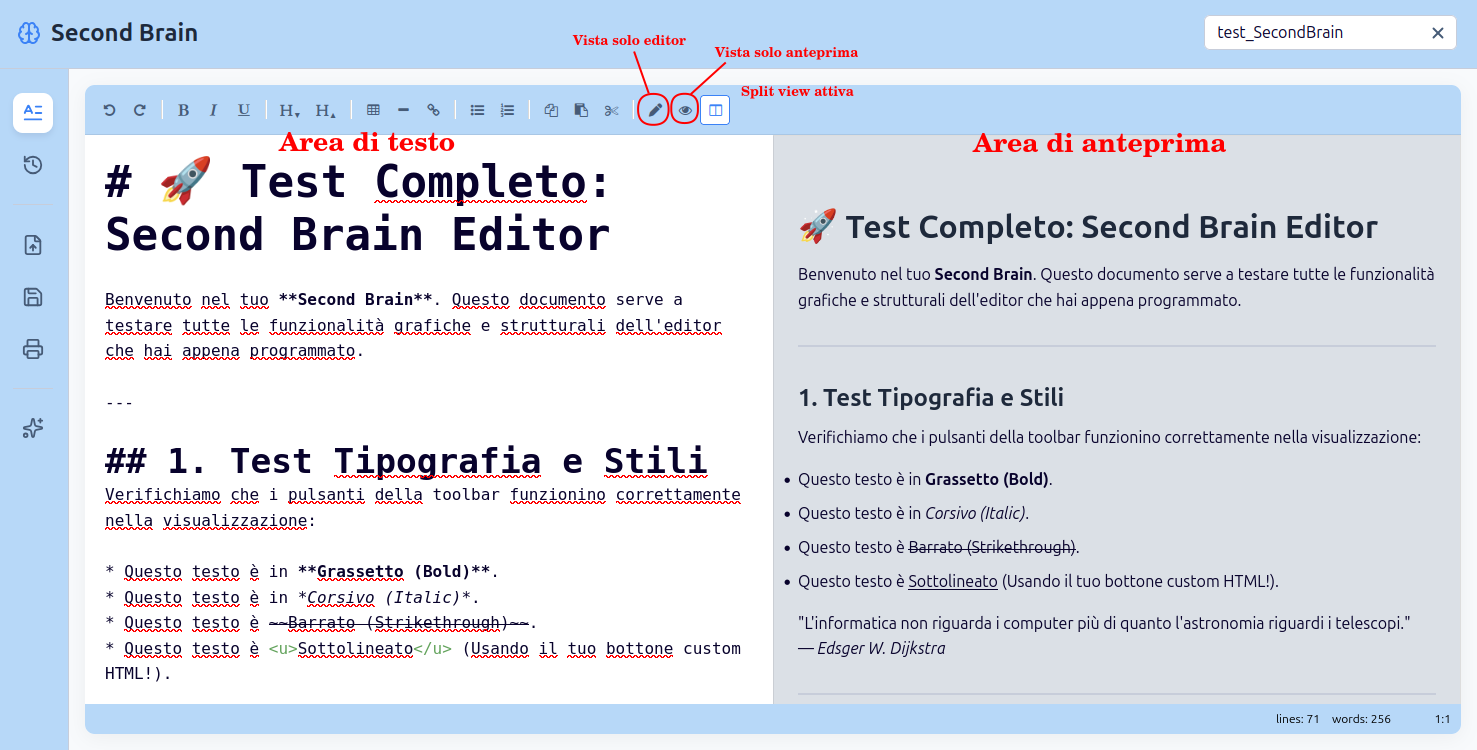
\includegraphics[width=1\textwidth]{../ManualeUtenteimg/split_view.png}
    \caption{Vista in modalità split view: a sinistra l'area di scrittura, a destra l'area di visualizzazione dell'anteprima formattata.}
    \label{fig:split_view}
\end{figure}


% ===========================================
% GESTIONE DEI FILE
% ===========================================
\section{Funzionalità dell'editor: Operazioni sui file}
Oltre alla fase di scrittura, \textit{Second Brain} offre strumenti avanzati per l'importazione, l'esportazione e la stampa dei documenti, permettendo una gestione completa del flusso di lavoro digitale.

\subsection{Caricamento di documenti (.md, .txt)}
Il sistema permette di riprendere il lavoro su file già esistenti tramite due modalità di caricamento:

\subsubsection{Caricamento standard (Sidebar)}
Cliccando sull'icona di \textbf{Upload} nella \textit{Sidebar} sinistra, si aprirà la finestra di selezione file del sistema operativo. È possibile selezionare un file con estensione \texttt{.md} o \texttt{.txt}. Se l'area di scrittura non è vuota, il sistema chiederà conferma prima di procedere per evitare di perdere il testo attuale.

\subsubsection{Caricamento rapido (Drag-and-Drop)}
Oltre alla procedura di caricamento standard, l'interfaccia supporta il \textbf{trascinamento diretto} dei file (\textit{Drag-and-Drop}). È possibile importare un documento in formato \texttt{.md} o \texttt{.txt} trascinandolo dal proprio computer e rilasciandolo direttamente all'interno dell'area di scrittura. 

Per prevenire la perdita accidentale del lavoro in corso, il sistema richiederà sempre una conferma esplicita prima di sovrascrivere il testo esistente con il contenuto del nuovo file. L'utente riceverà un feedback immediato sull'esito dell'operazione tramite una notifica a comparsa (successo o errore di caricamento) posizionata nell'angolo in basso a destra dello schermo.

\begin{figure}[H]
    \centering
    
\includegraphics[width=0.4\textwidth]{../ManualeUtenteimg/avviso_successo_upload.png}
    \caption{Avvisso di caricamento file riuscito.}
    \label{fig:panoramica}
\end{figure}


\subsection{Esportazione e Salvataggio}
Per salvare il documento sul proprio computer, cliccare sull'icona \textbf{Salva/Esporta} nella \textit{Sidebar}. Si aprirà una finestra modale per configurare il download.

\begin{figure}[H]
    \centering
    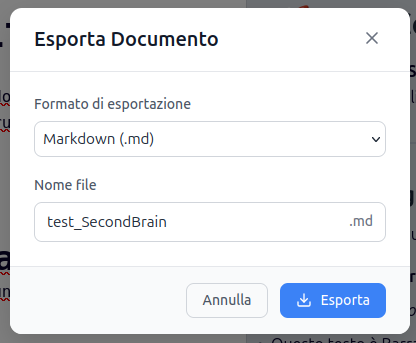
\includegraphics[width=0.5\textwidth]{../ManualeUtenteimg/modale_esportazione.png}
    \caption{Finestra di configurazione per l'esportazione del file.}
    \label{fig:modale_esportazione}
\end{figure}

Nella finestra di esportazione è possibile:
\begin{itemize}
    \item \textbf{Definire il nome del file}: Il sistema propone come predefinito il titolo impostato nella \textit{Topbar}, ma è possibile modificarlo liberamente prima del download.
    \item \textbf{Scegliere il formato}: Sono disponibili diversi formati per garantire la compatibilità con altri software:
    \begin{itemize}
        \item \textbf{Markdown (.md)}: Mantiene il codice sorgente originale.
        \item \textbf{Testo (.txt)}: Formato universale e leggero, ideale per salvare e leggere il contenuto testuale base su qualsiasi dispositivo.
        \item \textbf{HTML (.html)}: Per la pubblicazione diretta sul web.
    \end{itemize}
\end{itemize}

\begin{figure}[H]
    \centering
    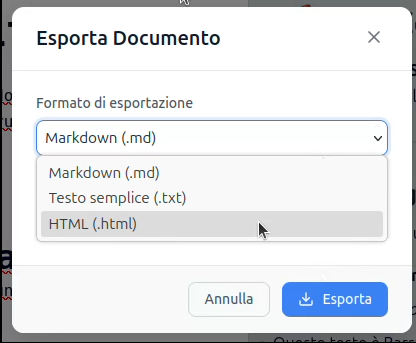
\includegraphics[width=0.5\textwidth]{../ManualeUtenteimg/modale_save.png}
    \caption{Possibili formati per l'esportazione del file.}
    \label{fig:formati_esportazione}
\end{figure}

Una volta confermata l'esportazione, il sistema visualizza una notifica di successo nell'angolo inferiore della schermata. Contemporaneamente, il browser avvia il download del file, il cui avanzamento può essere monitorato direttamente tramite la gestione dei download del programma di navigazione.

\begin{figure}[H]
    \centering
    % Prima immagine: Notifica di successo
    \begin{minipage}[b]{0.48\textwidth}
        \centering
        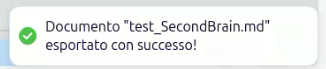
\includegraphics[width=\textwidth]{../ManualeUtenteimg/successo_save.png}
        \caption{Notifica di conferma esportazione.}
        \label{fig:successo_esportazione}
    \end{minipage}
    \hfill
    % Seconda immagine: Gestore download browser
    \begin{minipage}[b]{0.48\textwidth}
        \centering
        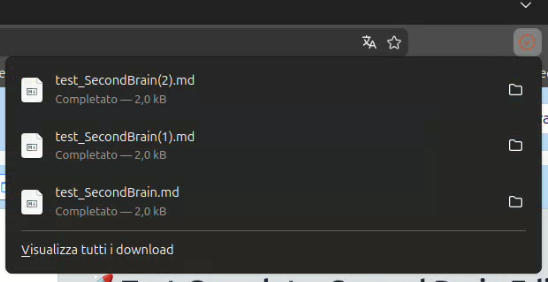
\includegraphics[width=\textwidth]{../ManualeUtenteimg/download.png}
        \caption{Monitoraggio del download nel browser.}
        \label{fig:download_file}
    \end{minipage}
\end{figure}


\subsection{Stampa del documento}
L'icona della stampante nella \textit{Sidebar} avvia il processo di stampa del browser. Il sistema applica automaticamente uno stile (\textit{Print Stylesheet}) che rimuove tutti gli elementi dell'interfaccia di \textit{Second Brain} (pulsanti, menu e barre laterali), garantendo che su carta o su file PDF appaia solo il testo del documento correttamente formattato, cioè solo l'anteprima del file formattato.

\begin{figure}[H]
    \centering
    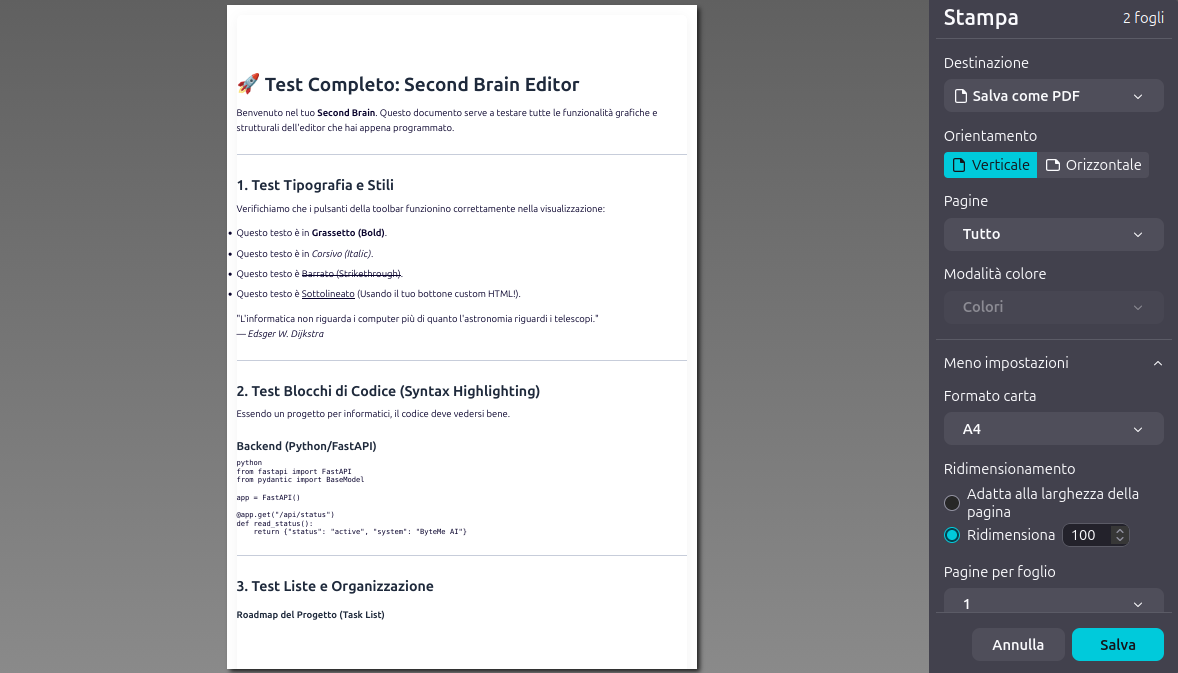
\includegraphics[width=1\textwidth]{../ManualeUtenteimg/stampa.png}
    \caption{Finestra del browser per configurare le impostazioni di stampa del documento.}
    \label{fig:stampa}
\end{figure}


\newpage

% ===================================================
% FUNZIONALITÀ DI INTELLIGENZA ARTIFICIALE
% ===================================================
\section{Funzionalità di Intelligenza Artificiale}
L'integrazione con l'Intelligenza Artificiale (AI) rappresenta il nucleo di \textit{Second Brain}. Il sistema non si limita a generare testo, ma agisce come un assistente editoriale capace di analizzare, tradurre e rielaborare i tuoi contenuti in modo contestuale.

\subsection{Attivazione e selezione del contenuto}
L'AI può operare in due modalità distinte in base alla tua necessità:
\begin{enumerate}
    \item \textbf{Selezione specifica}: Evidenzia con il mouse la porzione di testo che desideri elaborare. In questo caso, l'AI concentrerà la sua analisi esclusivamente su quel frammento.
    \item \textbf{Documento intero}: Se non viene effettuata alcuna selezione, l'AI utilizzerà come contesto l'intero contenuto presente nell'editor.
\end{enumerate}
Una volta definito il contenuto, clicca sull'icona \textbf{Azioni AI} nella \textit{Sidebar} per aprire il pannello degli strumenti.

\begin{figure}[H]
    \centering
    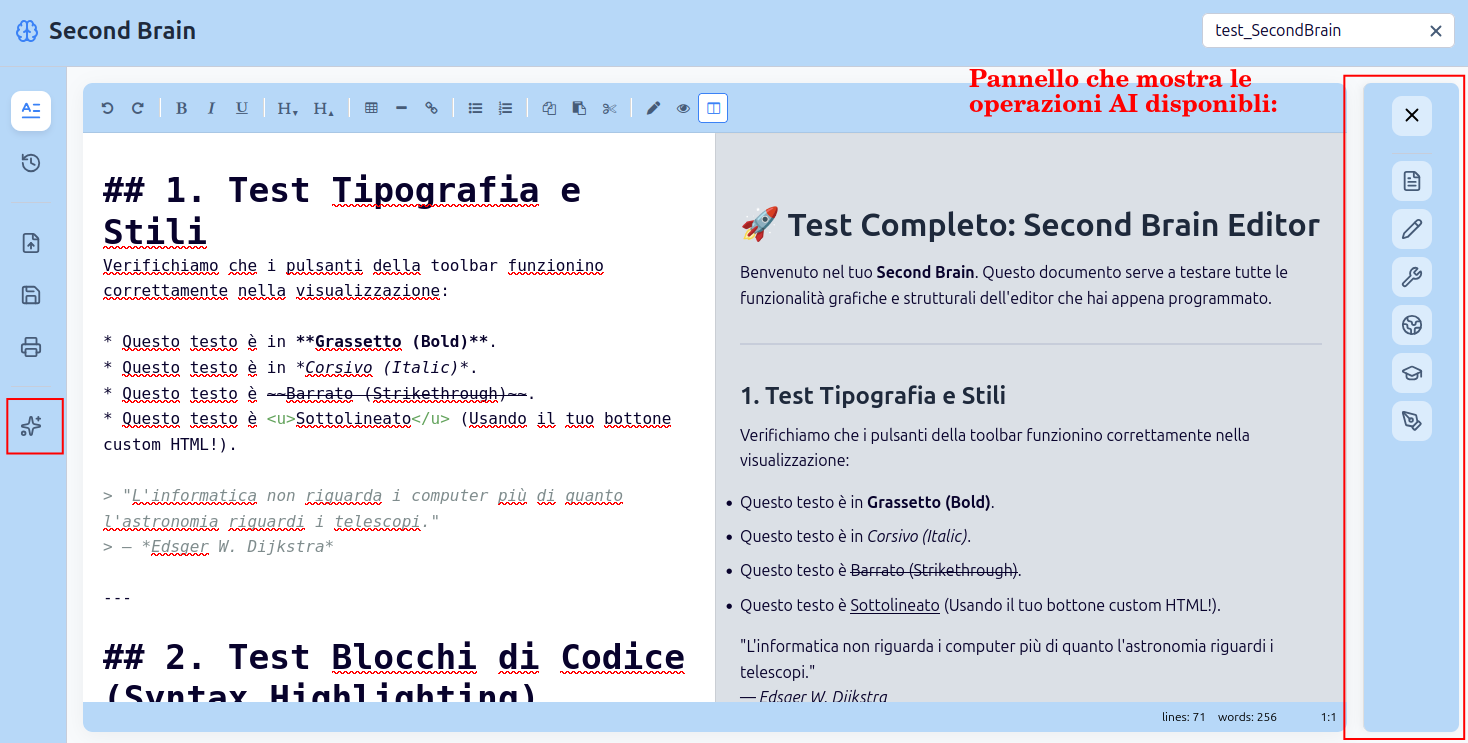
\includegraphics[width=1\textwidth]{../ManualeUtenteimg/pannelloAI.png}
    \caption{Pannello laterale che mostra le operazioni AI disponibili.}
    \label{fig:pannello_ai}
\end{figure}

% DESCRIZIONE OPERAZIONI
\subsection{Operazioni disponibili}
Il pannello AI di \textit{Second Brain} raccoglie una suite di strumenti progettati per potenziare ogni fase della produzione testuale. Le operazioni sono raggruppate in categorie intuitive per facilitare la scelta in base all'obiettivo editoriale.

\subsection{Strumenti editoriali}
Queste funzioni sono dedicate al raffinamento e all'ottimizzazione di contenuti già presenti nell'editor.
\begin{itemize}
    \item \textbf{Riassunto del testo}: L'AI analizza il contenuto e ne estrae i concetti fondamentali, producendo una sintesi densa ma leggibile. È lo strumento ideale per trasformare verbali lunghi, articoli complessi o appunti sparsi in paragrafi concisi che mantengono intatto il messaggio originale.
    \item \textbf{Correzione del testo}: Questa funzione agisce come un correttore di bozze evoluto. Non si limita a individuare refusi, ma analizza la concordanza grammaticale, la sintassi e la punteggiatura. L'intervento è conservativo: l'AI corregge gli errori formali senza alterare il tono di voce o il vocabolario scelto dall'utente.
    \item \textbf{Riscrittura del testo}: A differenza della correzione, la riscrittura interviene sullo stile. Rielabora le frasi per aumentarne la fluidità e l'eleganza formale. È particolarmente utile per trasformare una bozza scritta velocemente in un testo dal registro più professionale o accademico, migliorando la varietà lessicale.
\end{itemize}

\subsection{Traduzione multilingua}
Lo strumento di traduzione è progettato per superare le barriere linguistiche preservando il contesto tecnico del documento.
\begin{itemize}
    \item \textbf{Funzionamento}: Selezionando una lingua tra quelle supportate (Inglese, Spagnolo, Francese, Tedesco, Cinese), il sistema avvia una traduzione semantica.
    \item \textbf{Qualità}: A differenza dei traduttori letterali, l'AI di \textit{Second Brain} mantiene la coerenza delle terminologie specifiche e adatta le strutture sintattiche alla lingua di destinazione, garantendo un risultato naturale e pronto per la condivisione internazionale.
\end{itemize}

\subsection{Analisi critica con i "Sei Cappelli per Pensare"}
Questa sezione implementa il celebre metodo di Edward de Bono per il pensiero laterale. L'AI analizza il testo assumendo sei diverse "identità" critiche, offrendo all'utente una visione a 360 gradi di un'idea o di un progetto:
\begin{itemize}
    \item \textbf{Cappello Bianco (Fatti)}: Si concentra esclusivamente sui dati oggettivi, le informazioni disponibili e le evidenze concrete contenute nel testo.
    \item \textbf{Cappello Rosso (Emozioni)}: Estrapola la componente emotiva, le reazioni viscerali e le intuizioni, utile per valutare l'impatto psicologico di una proposta.
    \item \textbf{Cappello Nero (Criticità)}: Identifica i punti deboli, i rischi potenziali e le possibili ragioni per cui un'idea potrebbe fallire. Agisce come l'avvocato del diavolo.
    \item \textbf{Cappello Giallo (Ottimismo)}: Ricerca i benefici, il valore aggiunto e le opportunità positive, aiutando a vedere il potenziale di crescita.
    \item \textbf{Cappello Verde (Creatività)}: Propone alternative insolite, nuove direzioni e soluzioni creative partendo dagli spunti presenti nel testo.
    \item \textbf{Cappello Blu (Organizzazione)}: Fornisce una sintesi strutturata e una visione d'insieme, definendo le priorità e i passi successivi logici.
\end{itemize}

\subsection{Distant Writing (Generazione da zero)}
Il \textit{Distant Writing} è lo strumento dedicato alla creazione di nuovi contenuti. 
\begin{itemize}
    \item \textbf{Processo}: Attivando questa funzione, comparirà una finestra di input dove l'utente può inserire un'istruzione (prompt) descrivendo ciò che desidera ottenere (es: "Scrivi un'email formale di sollecito per una fattura scaduta").
    \item \textbf{Risultato}: L'AI elabora l'input e propone un testo completo, strutturato e pronto per essere inserito nell'editor. Se il risultato non soddisfa pienamente, è possibile utilizzare la funzione \textbf{Rigenera} per ottenere una variante diversa mantenendo la stessa istruzione originale.
\end{itemize}

% WIDGET
\subsection{AI Widget: integrità e controllo}
Il sistema \textit{Second Brain} è progettato per garantire all'utente il controllo totale sul proprio documento. Per questo motivo, l'Intelligenza Artificiale non sovrascrive mai direttamente il testo. Ogni risposta viene presentata all'interno di un \textbf{AI Widget}, un componente flottante che agisce come un'area di revisione temporanea.

\subsubsection{Caratteristiche del Widget}
\begin{itemize}
    \item \textbf{Interfaccia non bloccante}: Il widget è "trascinabile" (\textit{draggable}). Cliccando e trascinando la parte superiore del componente, è possibile spostarlo in qualsiasi punto della finestra per non coprire il testo che si sta consultando.
    \item \textbf{Sicurezza del contenuto}: Il testo all'interno del widget è in modalità "sola lettura". Non può essere modificato finché non viene confermato e inserito nell'editor; questo garantisce che la proposta dell'AI rimanga integra durante la fase di valutazione.
    \item \textbf{Isolamento dell'anteprima}: Finché l'utente non accetta la proposta, il testo generato non apparirà nell'area di anteprima (\textit{Preview}), assicurando che il documento "ufficiale" contenga solo dati verificati.
\end{itemize}

\begin{figure}[H]
    \centering
    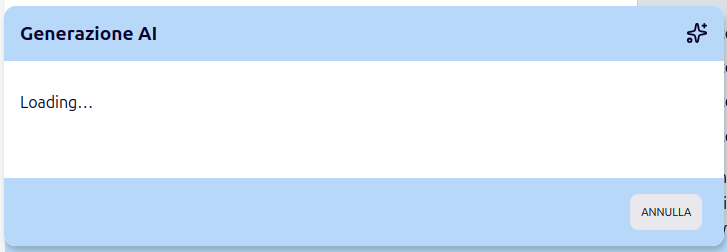
\includegraphics[width=0.6\textwidth]{../ManualeUtenteimg/widget_loading.png}
    \caption{Il widget nello stato di caricamento (\textit{Loading}): l'AI sta elaborando la richiesta.}
    \label{fig:ai_widget_loading}
\end{figure}

\subsubsection{Comandi di gestione}
Una volta che l'AI ha completato l'elaborazione, il widget espone tre opzioni operative:
\begin{itemize}
    \item \textbf{Inserisci}: Conferma la bontà del risultato. Se era stato selezionato del testo, questo verrà sostituito dalla proposta AI; in assenza di selezione, il nuovo testo verrà aggiunto immediatamente dopo la posizione del cursore.
    \item \textbf{Scarta}: Rifiuta la proposta e chiude il widget. Il documento originale rimane totalmente inalterato.
    \item \textbf{Rigenera}: Se il risultato non è soddisfacente, questo comando invia nuovamente la richiesta all'AI per ottenere una variante diversa, mantenendo lo stesso contesto o le stesse istruzioni.
\end{itemize}

\subsection{Distant Writing: generazione creativa}
La funzione \textbf{Distant Writing} è dedicata alla creazione di nuovi contenuti a partire da un'idea o un'istruzione specifica. A differenza degli strumenti editoriali, questa modalità richiede un input testuale diretto (\textit{prompt}) da parte dell'utente.

\paragraph{Procedura di utilizzo}
\begin{enumerate}
    \item Posiziona il cursore nell'editor nel punto esatto dove desideri che il testo venga generato.
    \item Apri il pannello AI e seleziona \textbf{Distant Writing}.
    \item Scrivi un prompt, un'istruzione o un'idea nel campo dedicato.
    \item Clicca su invia: il sistema mostrerà il widget di caricamento e, successivamente, la proposta testuale pronta per essere inserita o rigenerata.
\end{enumerate}

\begin{figure}[H]
    \centering
    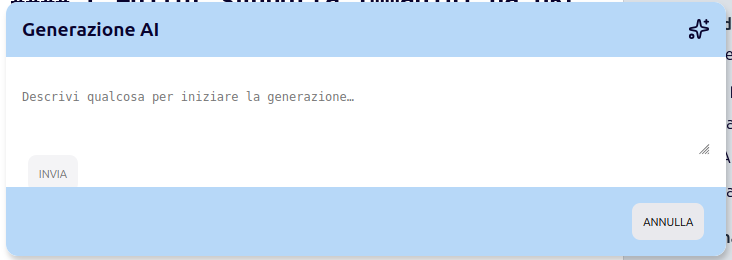
\includegraphics[width=0.6\textwidth]{../ManualeUtenteimg/widget_distant_writing.png}
    \caption{Interfaccia di input per il Distant Writing.}
    \label{fig:ai_widget_distant_writing}
\end{figure}

\subsection{Gestione degli stati di errore}
In caso di problemi di rete, timeout del server o interruzione della comunicazione con i modelli linguistici, il sistema entra in uno stato di sicurezza (\textit{Error State}). In questa condizione, il widget informa l'utente sulla natura del problema. 

L'unica azione consentita è il comando \textbf{Chiudi/Scarta}, che permette di resettare il widget e tornare allo stato di riposo, evitando che l'interfaccia rimanga bloccata in un'operazione fallita.

\begin{figure}[H]
    \centering
    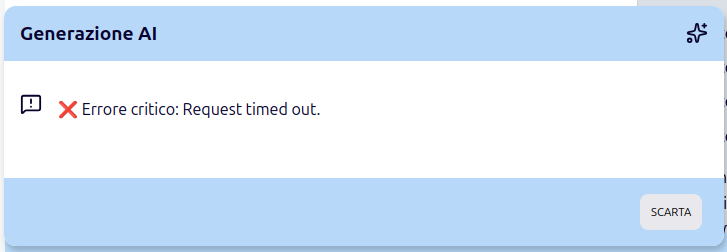
\includegraphics[width=0.5\textwidth]{../ManualeUtenteimg/widget_error.png}
    \caption{Feedback visivo del widget in caso di errore di sistema.}
    \label{fig:ai_widget_error}
\end{figure}


\newpage
% ===================================================
% STORICO DELLE GENERAZIONI
% ===================================================
\section{Storico delle generazioni AI}
Lo Storico delle generazioni AI è lo strumento di memoria del sistema. Ogni interazione con l'Intelligenza Artificiale che produce un risultato viene automaticamente archiviata per permettere consultazioni future, confronti tra diverse versioni o il recupero di testi scartati durante la sessione di scrittura.

\subsection{Accesso e navigazione}
Per visualizzare l'archivio, cliccare sull'icona dello storico presente nella Sidebar. L'editor verrà temporaneamente nascosto per lasciare spazio alla dashboard dello storico. È possibile tornare all'editor in qualsiasi momento cliccando nuovamente sull'icona della penna nella barra laterale.

\begin{figure}[H]
    \centering
    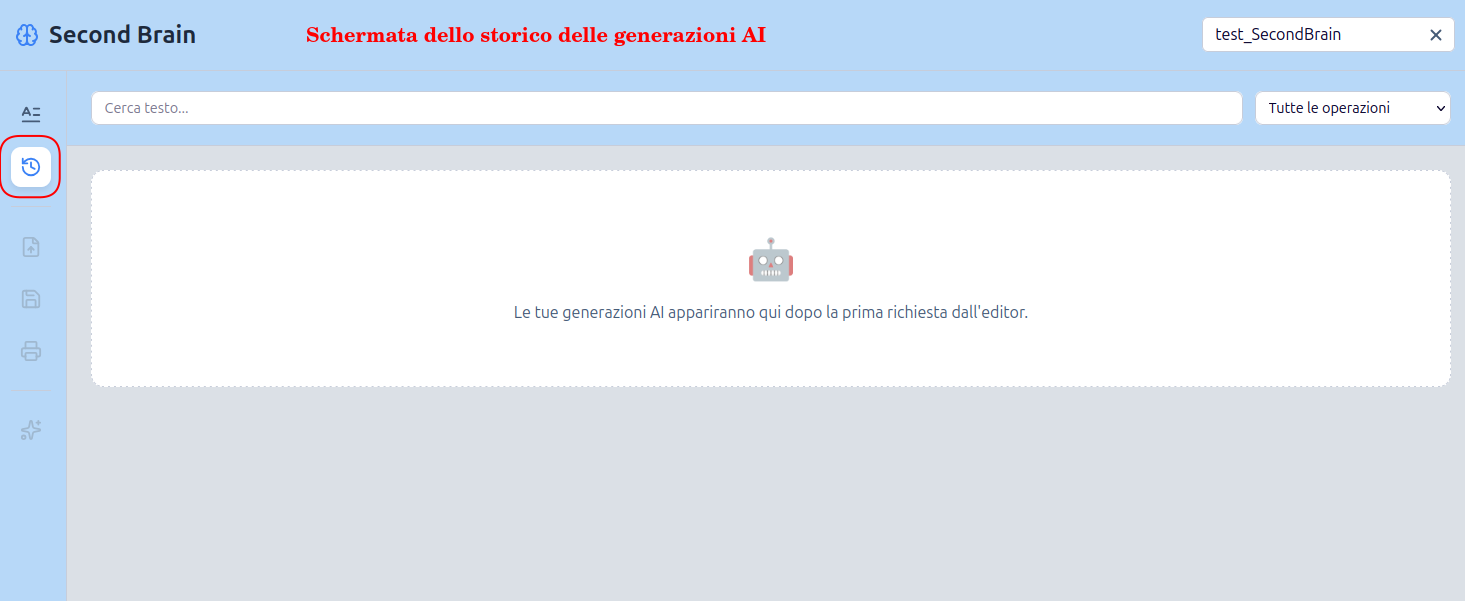
\includegraphics[width=1\textwidth]{../ManualeUtenteimg/storico_vuoto.png}
    \caption{Vista della dashboard dello storico al primo accesso, priva di generazioni archiviate.}
    \label{fig:storico}
\end{figure}


\subsection{Ricerca e filtraggio}
Per gestire volumi elevati di generazioni, la pagina offre strumenti di ricerca e filtraggio situati nella barra superiore della vista storico.

\begin{itemize}
    \item \textbf{Ricerca testuale}: Tramite la barra di ricerca è possibile filtrare i risultati in tempo reale inserendo parole chiave. Il sistema cercherà le corrispondenze sia all'interno del \textit{testo di input} (la richiesta originale) che nel \textit{testo generato}.
    \item \textbf{Filtro per operazione}: Un menu a tendina permette di isolare solo specifiche tipologie di attività. È possibile visualizzare, ad esempio, esclusivamente le traduzioni o solo le analisi effettuate con i "Sei Cappelli", nascondendo temporaneamente tutto il resto.
\end{itemize}

\begin{figure}[H]
    \centering
    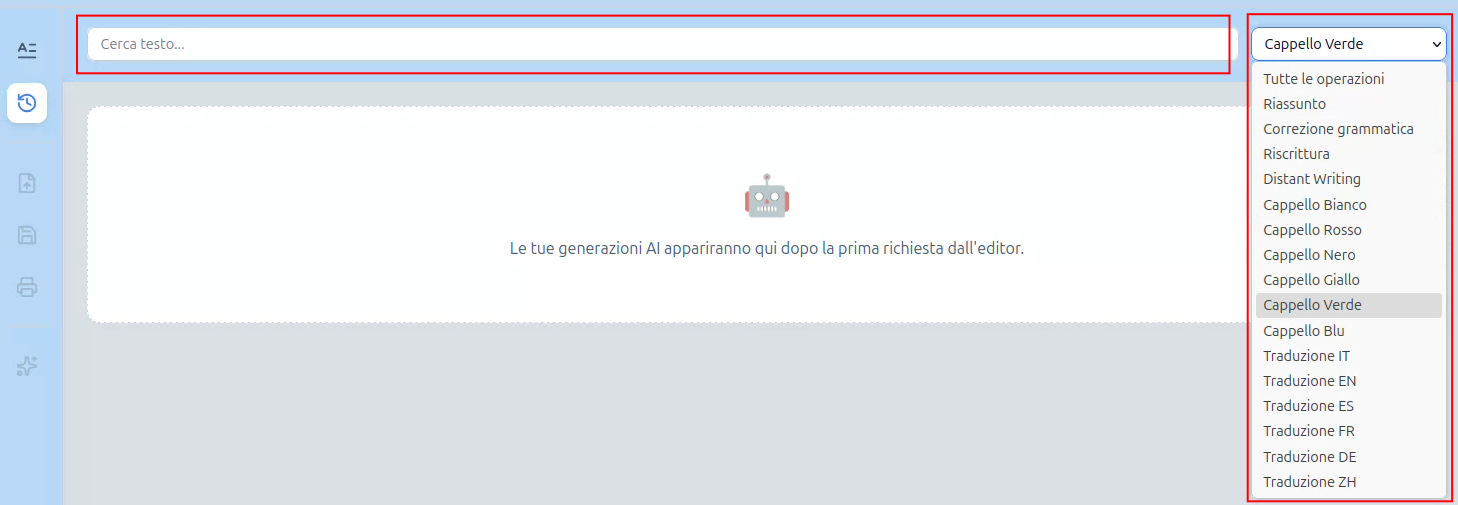
\includegraphics[width=1\textwidth]{../ManualeUtenteimg/filtri_storico.png}
    \caption{Strumenti di ricerca e filtraggio per la consultazione rapida delle generazioni archiviate.}
    \label{fig:filtri_storico}
\end{figure}


\subsection{Ordinamento e Visualizzazione}
Il sistema applica un ordinamento **cronologico decrescente**: le generazioni più recenti compaiono sempre in cima alla lista. Questo permette di avere immediatamente sottomano gli ultimi risultati ottenuti senza dover scorrere l'intero archivio.

\subsection{Caratteristiche delle singole generazioni presenti nello storico}
Ogni voce dello storico è racchiusa in una scheda informativa dettagliata che espone:
\begin{itemize}
    \item \textbf{Intestazione}: Mostra l'icona e il nome dell'operazione eseguita e il timestamp esatto (data e ora).
    \item \textbf{Risultato}: Il corpo principale della scheda che contiene il testo generato. Da qui è possibile selezionare e copiare il testo per riutilizzarlo nell'editor.
\end{itemize}

% screenshoot esempio di una generazione

\subsection{Gestione della memoria locale}
Le generazioni occupano spazio nella memoria del browser. Sebbene il sistema sia ottimizzato per gestire centinaia di voci, è possibile gestire la pulizia dei dati:
\begin{itemize}
    \item \textbf{Eliminazione singola}: Ogni scheda dispone di un'icona (cestino) per rimuovere definitivamente quella specifica generazione.
\end{itemize}

\textit{Nota sulla sicurezza}: Lo storico è strettamente legato al browser in uso. Se si utilizza la modalità di navigazione in incognito, lo storico verrà cancellato automaticamente alla chiusura della finestra. Per conservare i risultati a lungo termine, si consiglia di esportare periodicamente i documenti principali.


\newpage
% =================================================
% RISOLUZIONE DEI PROBLEMI (FAQ)
% =================================================
\section{Risoluzione dei problemi (FAQ)}
Di seguito sono elencate le soluzioni ai problemi più comuni in cui potresti incorrere durante l'installazione o l'utilizzo di \textit{Second Brain}.

\subsection{Problemi di installazione e avvio}

\paragraph{\gls{Docker} mostra un errore di "Porta già in uso" (Port already allocated)}
Questo accade quando un'altra applicazione sul tuo computer sta già utilizzando la porta \texttt{8080} (necessaria per l'interfaccia) o la \texttt{8000} (necessaria per il server).
\begin{itemize}
    \item \textbf{Soluzione}: Interrompi l'applicazione in conflitto, oppure apri il file \texttt{docker-compose.yml} con un editor di testo e modifica il parametro \texttt{ports} (es. da \texttt{"8080:8080"} a \texttt{"8081:8080"}). Successivamente, ripeti il comando di avvio e accedi a \texttt{http://localhost:8081}.
\end{itemize}

\paragraph{Il terminale mostra l'errore "docker-compose command not found"}
L'installazione di \gls{Docker} Desktop potrebbe non essere andata a buon fine o le variabili d'ambiente del tuo sistema operativo non sono aggiornate.
\begin{itemize}
    \item \textbf{Soluzione}: Assicurati che l'applicazione \gls{Docker} Desktop sia aperta e in esecuzione in background prima di digitare i comandi nel terminale. Se utilizzi una versione molto recente, prova a digitare \texttt{docker compose} (senza il trattino).
\end{itemize}

\subsection{Problemi durante l'utilizzo}

\paragraph{L'Intelligenza Artificiale risponde con uno stato di errore continuo}
Se il widget restituisce immediatamente un errore ogni volta che si avvia un'operazione, il server non riesce a comunicare con il provider linguistico.
\begin{itemize}
    \item \textbf{Soluzione 1}: Verifica di aver creato correttamente il file \texttt{.env} nella cartella principale e di aver inserito chiavi API valide, come spiegato nel capitolo di Installazione. Se hai modificato il file \texttt{.env} a sistema già avviato, devi riavviare l'applicazione (\texttt{Ctrl + C} nel terminale, seguito nuovamente da \texttt{docker-compose up --build}).
    \item \textbf{Soluzione 2}: Assicurati che il tuo computer sia connesso a Internet. Sebbene il software funzioni localmente, le operazioni AI richiedono una connessione attiva per interrogare i modelli LLM.
\end{itemize}

\paragraph{Ho aperto l'applicazione ma il mio documento precedente è scomparso}
Se hai cambiato browser (es. passata da Chrome a Firefox), hai aperto una finestra di navigazione in incognito, oppure hai svuotato la cache del browser, il sistema non troverà i dati precedenti.
\begin{itemize}
    \item \textbf{Soluzione}: I dati non esportati manualmente vivono solo nella memoria locale di quella specifica finestra di quel specifico browser. Ricordati sempre di utilizzare l'icona "Salva/Esporta" nella \textit{Sidebar} per salvare copie fisiche in formato \texttt{.md} dei tuoi lavori più importanti sul computer.
\end{itemize}


\end{document}